\iffalse
\documentclass[]{article}
\usepackage{amsfonts, amssymb, amsmath}
\usepackage{float}
\usepackage{graphicx}

\title{Question 10.13.3.1}
\author{Umair Parwez \\ EE22BTECH11009}
\date{}
\begin{document}
\maketitle
\providecommand{\pr}[1]{\ensuremath{\Pr\left(#1\right)}}
\providecommand{\prt}[2]{\ensuremath{p_{#1}^{\left(#2\right)} }}        % own macro for this question
\providecommand{\qfunc}[1]{\ensuremath{Q\left(#1\right)}}
\providecommand{\sbrak}[1]{\ensuremath{{}\left[#1\right]}}
\providecommand{\lsbrak}[1]{\ensuremath{{}\left[#1\right.}}
\providecommand{\rsbrak}[1]{\ensuremath{{}\left.#1\right]}}
\providecommand{\brak}[1]{\ensuremath{\left(#1\right)}}
\providecommand{\lbrak}[1]{\ensuremath{\left(#1\right.}}
\providecommand{\rbrak}[1]{\ensuremath{\left.#1\right)}}
\providecommand{\cbrak}[1]{\ensuremath{\left\{#1\right\}}}
\providecommand{\lcbrak}[1]{\ensuremath{\left\{#1\right.}}
\providecommand{\rcbrak}[1]{\ensuremath{\left.#1\right\}}}
\newcommand{\sgn}{\mathop{\mathrm{sgn}}}
\providecommand{\abs}[1]{\left\vert#1\right\vert}
\providecommand{\res}[1]{\Res\displaylimits_{#1}} 
\providecommand{\norm}[1]{\left\lVert#1\right\rVert}
%\providecommand{\norm}[1]{\lVert#1\rVert}
\providecommand{\mtx}[1]{\mathbf{#1}}
\providecommand{\mean}[1]{E\left[ #1 \right]}
\providecommand{\cond}[2]{#1\middle|#2}
\providecommand{\fourier}{\overset{\mathcal{F}}{ \rightleftharpoons}}
\newenvironment{amatrix}[1]{%
  \left(\begin{array}{@{}*{#1}{c}|c@{}}
}{%
  \end{array}\right)
}
%\providecommand{\hilbert}{\overset{\mathcal{H}}{ \rightleftharpoons}}
%\providecommand{\system}{\overset{\mathcal{H}}{ \longleftrightarrow}}
	%\newcommand{\solution}[2]{\textbf{Solution:}{#1}}
\newcommand{\solution}{\noindent \textbf{Solution: }}
\newcommand{\cosec}{\,\text{cosec}\,}
\providecommand{\dec}[2]{\ensuremath{\overset{#1}{\underset{#2}{\gtrless}}}}
\newcommand{\myvec}[1]{\ensuremath{\begin{pmatrix}#1\end{pmatrix}}}
\newcommand{\mydet}[1]{\ensuremath{\begin{vmatrix}#1\end{vmatrix}}}
\newcommand{\myaugvec}[2]{\ensuremath{\begin{amatrix}{#1}#2\end{amatrix}}}
\providecommand{\rank}{\text{rank}}
\providecommand{\pr}[1]{\ensuremath{\Pr\left(#1\right)}}
\providecommand{\qfunc}[1]{\ensuremath{Q\left(#1\right)}}
	\newcommand*{\permcomb}[4][0mu]{{{}^{#3}\mkern#1#2_{#4}}}
\newcommand*{\perm}[1][-3mu]{\permcomb[#1]{P}}
\newcommand*{\comb}[1][-1mu]{\permcomb[#1]{C}}
\providecommand{\qfunc}[1]{\ensuremath{Q\left(#1\right)}}
\providecommand{\gauss}[2]{\mathcal{N}\ensuremath{\left(#1,#2\right)}}
\providecommand{\diff}[2]{\ensuremath{\frac{d{#1}}{d{#2}}}}
\providecommand{\myceil}[1]{\left \lceil #1 \right \rceil }
\newcommand\figref{Fig.~\ref}
\newcommand\tabref{Table~\ref}
\newcommand{\sinc}{\,\text{sinc}\,}
\newcommand{\rect}{\,\text{rect}\,}
%%
%	%\newcommand{\solution}[2]{\textbf{Solution:}{#1}}
%\newcommand{\solution}{\noindent \textbf{Solution: }}
%\newcommand{\cosec}{\,\text{cosec}\,}
%\numberwithin{equation}{section}
%\numberwithin{equation}{subsection}
%\numberwithin{problem}{section}
%\numberwithin{definition}{section}
%\makeatletter
%\@addtoreset{figure}{problem}
%\makeatother

%\let\StandardTheFigure\thefigure
\let\vec\mathbf

Two dice are thrown at the same time. Determine the probabiity that the difference
of the numbers on the two dice is 2. 
\fi
\solution
Let X, Y and Z be random variables with definition given as under:
\begin{table}[H]
\centering
\begin{tabular}{|c|c|c|}
    \hline
    $X$ & Number appearing on the first dice & \\
    \hline
    $Y$ & Number appearing on the second dice & \\
    \hline
    $Z$ & Difference of the numbers appearing on the dice & X - Y\\
    \hline
\end{tabular}
\label{tab:ncert/10/13/3/1/}
\caption{Definition of Random variables.}
\end{table}

\begin{align}
    p_X(k) &= \frac{1}{6}\\
	p_Y(k) &= p_X(k) 
\end{align}
PMF of $W$ using $z$-transform:
applying the z-transform on both the sides
\begin{align}
	M_Z(z) &= M_{X-Y}(z)\\
	&= M_X(z)\cdot M_Y(z^{-1})\\
  &= \Sigma p_X(k)z^{-k} \cdot \Sigma p_Y(k)z^{k}\\
  &= \frac{1}{6}(z^{-1}+z^{-2}\nonumber+z^{-3}+z^{-4}+z^{-5}+z^{-6}) \cdot \frac{1}{6}(z+z^2 \\&\qquad +z^3+z^4+z^5+z^6) \\
  &= \frac{1}{36}(z^{-5}+2z^{-4}+3z^{-3}+4z^{-2}+5z^{-1}+6z^{0}\nonumber\\&\qquad+5z^{1}+4z^{2}+3z^{3}+2z^{4}+z^{5})
\end{align}
Now, we also know that, 
\begin{align}
	M_Z(z) &= \Sigma p_Z(k)z^{-k}
\end{align}
Therefore, 
\begin{align}
	\Sigma p_Z(k)z^{-k} &= \frac{1}{36}(z^{-5}+2z^{-4}+3z^{-3}+4z^{-2}+5z^{-1}+6z^{0}\nonumber\\&\qquad+5z^{1}+4z^{2}+3z^{3}+2z^{4}+z^{5}) \label{eq:pmf}
\end{align}
From \eqref{eq:pmf}, we can extract the PMF of Z.

Now, let $E$ be the event that the difference of the numbers on the two dice is 2. Then,
\begin{align}
  p(E) = p_Z(2) +p_Z(-2)\\
\end{align}
From \eqref{eq:pmf}, we find that,
\begin{align}
  p_Z(2) = \frac{1}{9} \\
  p_Z(-2) = \frac{1}{9}
\end{align}
Therefore,
\begin{align}
  p(E)=\frac{2}{9}
\end{align}
Shown below is a graph visualising a simulation of the given question, with the 2 dice being rolled 10,000 times and comparing it to the theoretical probability
\begin{figure}[h]
  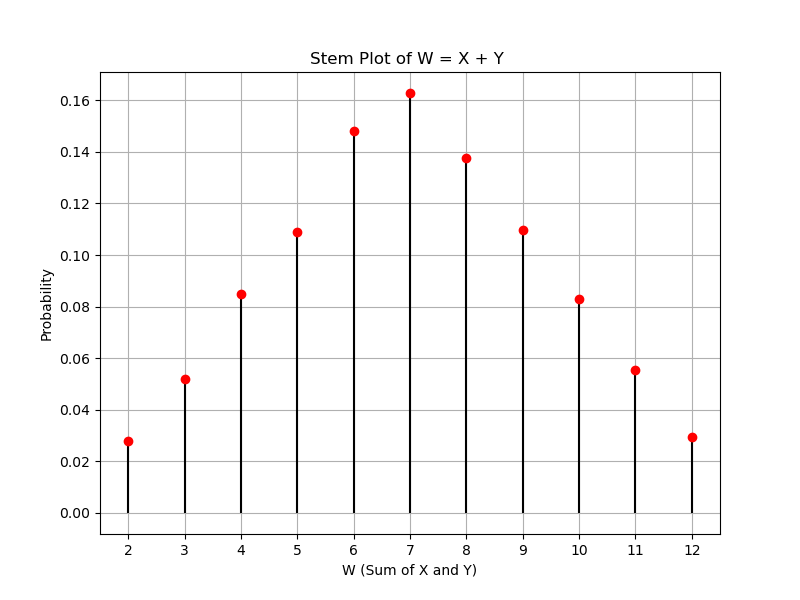
\includegraphics[width=\columnwidth]{./figs/Z.png}
  \caption{Stem plot for P(Z)}
  \label{fig:exemplar/10/13/3/1/Z/}
\end{figure}

